\documentclass{article}
\usepackage{graphicx}
\usepackage{subcaption}

\title{Side-by-Side Graphics}
\author{JSSATEB}
\date{\today}

\begin{document}
	\maketitle

	\section{Introduction}
		This section illustrates the use of Side-by-Side Graphics using Subfigure. Figures \ref{fig:image1} and \ref{fig:image2} are the subfigure under the title of Figure \ref{fig:sidebyside}.
		\begin{figure}[h!]
   			 \centering
    		\begin{subfigure}[b]{0.45\textwidth}
       			 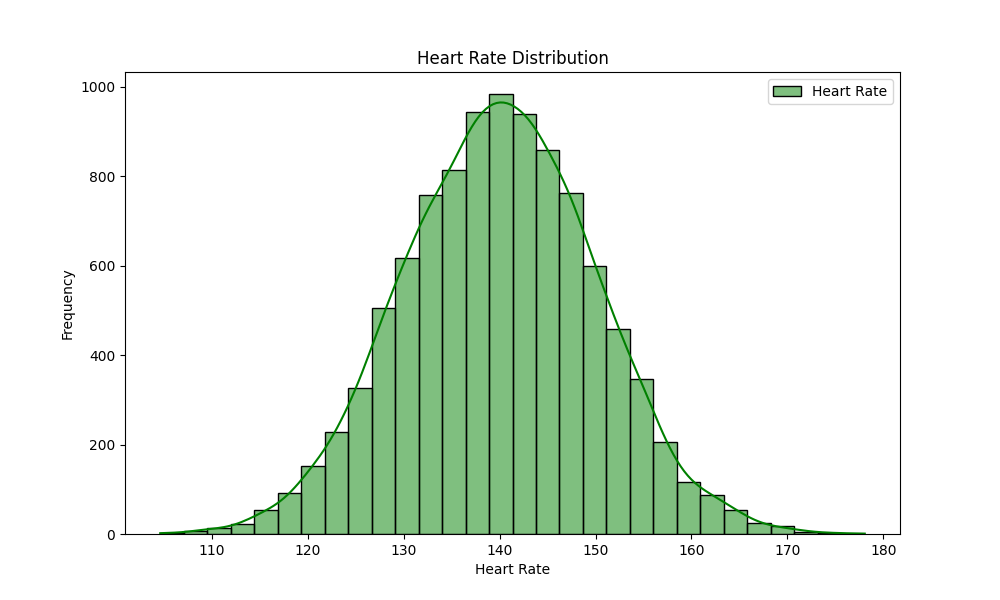
\includegraphics[width=\textwidth]{Individual prog heat.png}
       			 \caption{Image 1}
       			 \label{fig:image1}
   			 \end{subfigure}
   			 \begin{subfigure}[b]{0.45\textwidth}
       				 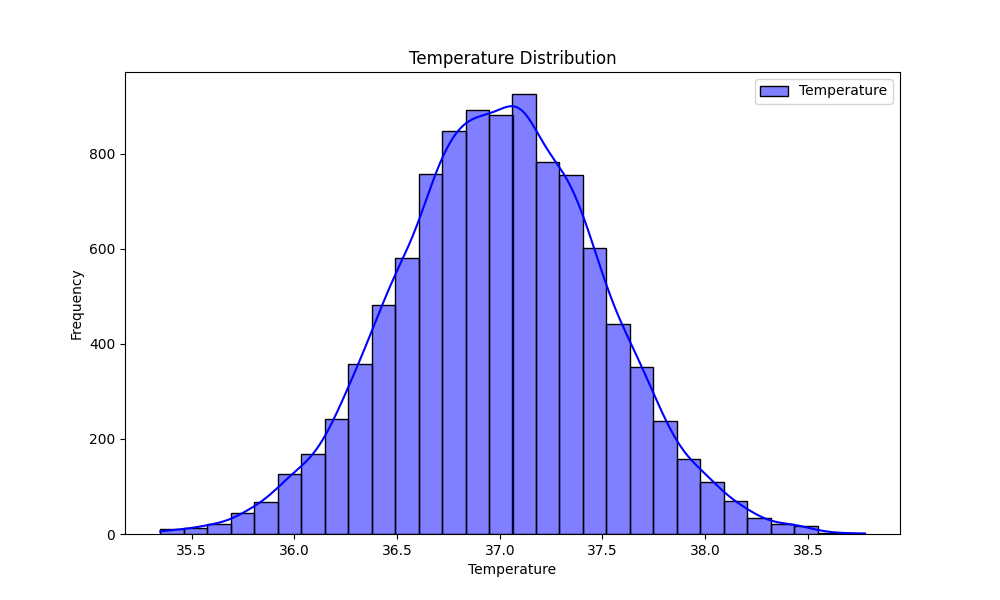
\includegraphics[width=\textwidth]{Temperature Distribution.png}
       				 \caption{Image 2}
       				 \label{fig:image2}
    		\end{subfigure}
    		\caption{Side-by-Side Images}
   			 \label{fig:sidebyside}
		\end{figure}

\end{document}
